\cleardoublepage
% \newpage
% \thispagestyle{empty}
% \mbox{}

\chapter{Optimización del rendimiento de OmpSs sobre arquitecturas asimétricas}
\label{ch:chapter4}

%\section{Descripción de la estrategia de optimización}
%
%\section{BLIS}
%
%\subsection{Adaptación de BLIS a arquitecturas asimétricas}
%
%\section{Combinación de BLIS asimétrico con OmpSs}
%
\section{Planteamiento general}

In this section, we initially perform an evaluation 
of the task-parallel Cholesky routine in Listings~\ref{lst:chol}--\ref{lst:chol_tasks},
executed on top of the conventional (i.e., default) scheduler in 
OmpSs linked to a sequential instance of BLIS,  on the target Exynos 5422 SoC.  The outcome from this study 
motivates the development effort and experiments presented in the remainder of the paper.

\subsection{Evaluación de runtimes convencionales en AMPs}

Figure~\ref{fig:ompss_blis_oversubscription} reports the performance,
in terms of GFLOPS (billions of flops per second), attained with the conventional OmpSs runtime,
when the number of worker threads varies from~1 to~8, and the mapping of worker threads to cores is delegated to the OS. 
We evaluated a range of block sizes
({\tt b} in Listing~\ref{lst:chol}), but for simplicity we report only the results obtained with the value {\tt b} that optimized
the GFLOPS rate for each problem dimension.
All the experiments hereafter employed {\sc ieee} double precision. Furthermore,
we  ensured that the cores operate at the highest possible frequency by setting the appropriate {\em cpufreq} governor.
The conventional runtime of OmpSs corresponds to release 15.06 of the Nanos++ runtime task scheduler.
For this experiment, it is lined with the ``sequential'' implementation of BLIS in release 0.1.5.
(For the experiments with the multi-threaded/asymmetric version of BLIS in the later sections, 
we will use specialized versions of the codes in~\cite{asymBLIS} for slow+fast VCs.)

%
The results in the
Figure reveal the increase in performance as the number of worker threads is raised from 1 to 4, which the OS maps
to the (big) Cortex-A15 cores. However, when the number of threads exceeds the amount of fast cores, the OS starts binding the threads
to the slower Cortex-A7 cores, and the improvement rate is drastically reduced, 
%(in part, due to the lower peak performance of the Cortex-A7 compared with the Cortex-A14) 
in some cases even showing a performance drop. This
is due to load imbalance, as tasks of uniform granularity, possibly laying in the critical path,
are assigned to slow cores. %Clearly, some type of asymmetry-awareness is necessary in the runtime task scheduler 
%(or the underlying libraries) in order to tackle this source of inefficiency.

\begin{figure}
\centering
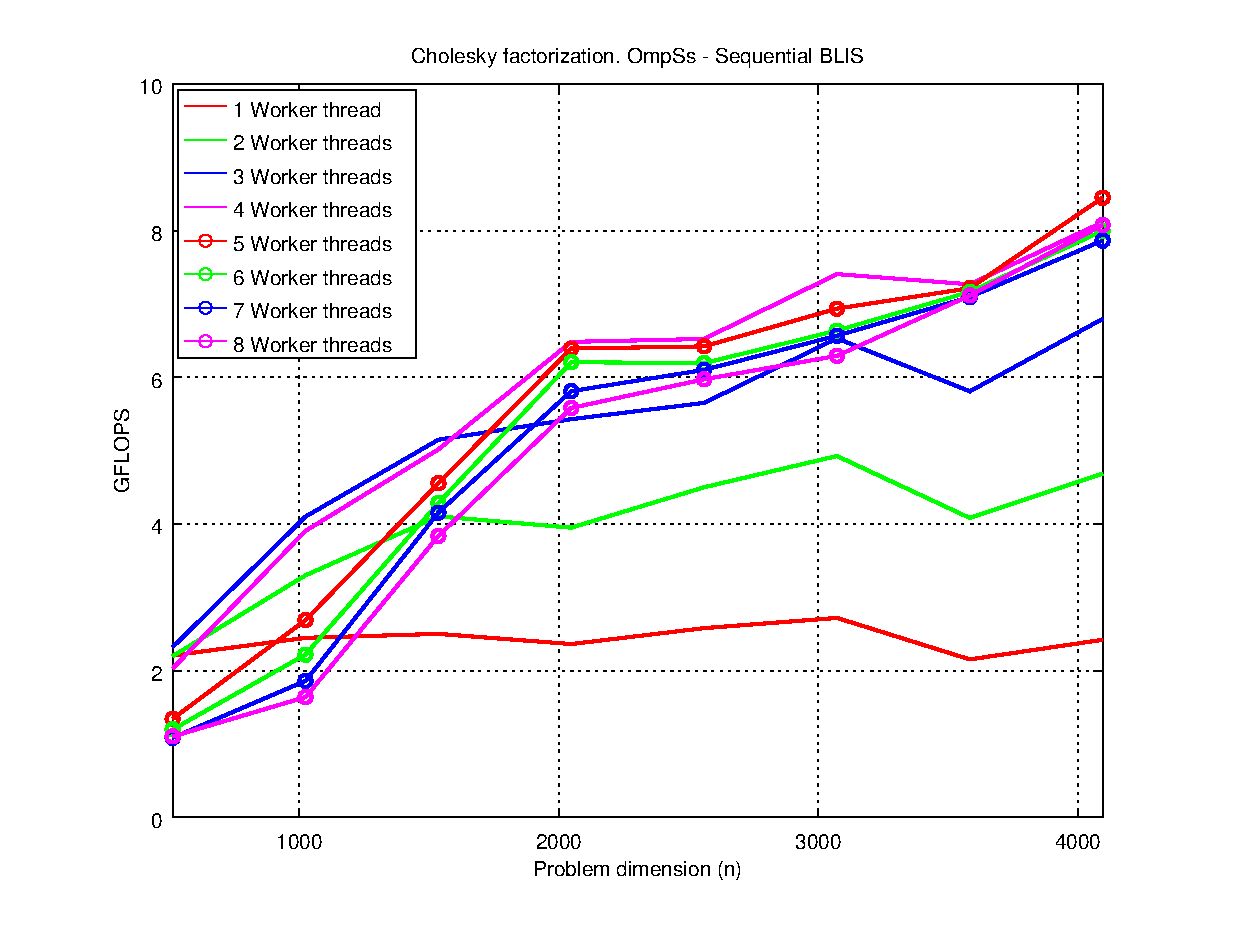
\includegraphics[width=0.70\textwidth]{Plots/Orig_runtime/plot_1to8_th}
\caption{Performance of the Cholesky factorization using the conventional OmpSs runtime and a sequential implementation
                 of BLIS on the Exynos 5422 SoC.}
\label{fig:ompss_blis_oversubscription}
\end{figure}

Stimulated by this first experiment, we recognize that an obvious solution to this problem consists in 
adapting the runtime task scheduler (more specifically, the scheduling policy) to exploit the 
SoC asymmetry~\cite{OmpSsbigLITTLE}.
Nevertheless, we part ways with this
solution, exploring an architecture-aware alternative
that leverages a(ny) conventional runtime task scheduler combined with an underlying asymmetric library. 
We discuss this option in more detail in the following section.

%%\subsection{Combining conventional runtimes with asymmetric libraries}
\section{Combinación de runtimes convencionales con bibliotecas asimétricas}

\subsection{General view}
Our proposal operates under the GTS model but is inspired in CPUM. Concretely,
our task scheduler regards
the computational resources as four {\em truly} symmetric VCs, each composed of a fast and a slow core. For this purpose, 
unlike CPUM, {\em both} physical cores within each VC remain active and collaborate to execute a given task.
Furthermore, our approach exploits concurrency at two levels: {\em task-level parallelism} is extracted by the runtime in order
to schedule tasks to the four symmetric VCs;
and each task/kernel is internally divided to 
expose {\em data-level parallelism}, distributing its workload between the two asymmetric physical cores within the VC
in charge of its execution.

Our solution thus only requires a conventional 
(and thus asymmetry-agnostic) runtime task scheduler, e.g. the conventional version of OmpSs, where instead of spawning one worker thread
per core in the system, we adhere to the CPUM model, creating only one worker thread per VC.
Internally, whenever a ready task is selected to be executed by a worker thread, 
the corresponding routine from BLIS internally spawns two threads, 
binds them to the appropriate pair of Cortex-A15+Cortex-A7 cores, 
and asymmetrically divides the work between the fast and the slow physical cores in the VC.
Following this idea, the architecture exposed to the runtime is {\em symmetric}, 
and the kernels in the BLIS library configure a ``black box'' that abstracts the 
architecture asymmetry from the runtime scheduler. 

In summary, in a conventional setup, the core is the basic computational resource for the task scheduler, 
and the ``sequential'' tasks are the minimum work unit to be assigned to these resources. Compared with this, in our approach the VC 
is the smallest (basic) computational resource from the point of view of the scheduler;
and tasks are further divided into smaller units, and executed in parallel by the physical cores inside the VCs.
%and parallel/asymmetric tasks are the minimum unit of work.

\subsection{Comparison with other approaches}
%Provided an underlying asymmetry-aware library is available to the developer, it is possible to combine this 
%with an existing conventional runtime task scheduler in order to exploit the underlying architecture. 
%In the enhanced version of OmpSs in~\cite{OmpSsbigLITTLE}, tasks were actually invocations to a {\em sequential} 
%library implementation, and asymmetry was exploited via sophisticated scheduling policies specially designed for asymmetric architectures. 
%Following our new approach, asymmetry is exploited at the library level, not at the runtime level. 
%To accommodate this, tasks are cast in terms of 
%invocations to a multi-threaded asymmetry-aware library (in our case, BLIS). 

Our approach features a number of advantages for the developer:
\begin{itemize}
\item The runtime is not aware of asymmetry, and thus a conventional task scheduler 
      will work transparently with no special modifications.
\item Any existing scheduling policy (e.g. cache-aware mapping or work stealing)
      in an asymmetry-agnostic runtime, or any enhancement technique, will directly impact the performance attained on an AMP.
\item Any improvement in the asymmetry-aware BLIS implementation will directly impact the performance on an AMP. 
      This applies to different ratios of big/LITTLE cores within a VC, operating frequency, or even to the introduction further levels
      of asymmetry (e.g. cores with a capacity between fast and slow).
\end{itemize}

Obviously, there is also a drawback in our proposal
as a tuned asymmetry-aware DLA library must exist in order to 
reuse conventional runtimes. 
In the scope of DLA, this drawback is easily tackled with BLIS. We recognize that, in more general domains, 
an ad-hoc implementation of the application's 
fundamental kernels becomes mandatory in order to fully exploit the underlying architecture.

%The implications and support necessary for this approach are explained next.

\subsection{Requisites on the BLAS-3}

We finally note that certain requirements are imposed on a multi-threaded implementation of BLIS that operates under the 
CPUM mode. 
To illustrate this, consider the \gemm kernel and the high-level description of its implementation
in Listing~\ref{lst:gemm}. For our objective,
we still have to distribute the iteration space between the Cortex-A15 and the Cortex-A7 but, since there is only one resource of each type per VC,
there is no need to partition the loops internal to the macro-kernel. 
Furthermore, we note that the optimal strides for Loop~1 are in practice quite
large ({\tt nc} is in the order of a few thousands for ARM big.LITTLE cores), while the optimal values for Loop~3 are much more reduced
({\tt mc} is 32 for the Cortex-A7 and 156 for the Cortex-A15). Therefore, we target Loop~3 in our data-parallel implementation of BLIS for
VCs, which we can expect to easily yield a proper workload balancing.

%That is, both the number of cores to use, and the distribution of those cores between the fast and slow processing units are transparent and 
%fully configurable by the user. 

\section{Resultados experimentales}

Let us start by reminding that, at execution time, OmpSs decomposes the routine for the Cholesky factorization into a collection of tasks 
that operate on sub-matrices (blocks) with a granularity 
dictated by the block size {\tt b}; see Listing~\ref{lst:chol}. 
These tasks typically perform invocations to a fundamental kernel of the BLAS-3, 
in our case provided by BLIS, or LAPACK; see Listing~\ref{lst:chol_tasks}.  

\newcommand{\bopt}{b^{\mbox{\rm \scriptsize opt}}\xspace}

The first step in our evaluation aims to provide a realistic estimation of the potential performance benefits
of our approach (if any) on the target Exynos 5422 SoC. 
A critical factor from this perspective is the range of block sizes, say $\bopt$,
that are optimal for the conventional OmpSs runtime. In particular, the efficiency 
of our hybrid task/data-parallel approach is strongly determined by the performance 
attained with the asymmetric BLIS implementation when compared against that of its sequential counterpart,
for problem dimensions {\tt n} that are in the order of $\bopt$.
%the optimal {\tt b} using the conventional OmpSs runtime.

Table~\ref{tab:optimal_bs_sym} reports the optimal block sizes $\bopt$ 
for the Cholesky factorization, with problems of increasing matrix dimension, using the conventional
OmpSs runtime linked with the sequential BLIS, and~1 to~4 worker threads.
Note that, except for smallest problems, the observed optimal block sizes
are between 192 and 448. These dimensions offer a 
fair compromise, exposing enough task-level parallelism
while delivering high ``sequential'' performance for the execution of each individual task
via the sequential implementation of BLIS.

%\begin{table}
	%\centering
	%\caption{Optimal block sizes for the Cholesky factorization using the sequential BLIS.}
	%\label{tab:optimal_bs_sym}
	%\begin{tabular}{|c||c|c|c|c|c|c|c|c|c|c|c|c|c|c|c|} 
		%\hline
		%Th. &     512 & 1024 & 1536 & 2048 & 2560 & 3072 & 3584 & 4096 & 4608 & 5120 & 5632 & 6144 & 6656 & 7168 & 7680 \\ \hline \hline
		%1   &     192 & 384 & 320 & 448 & 448 & 448 & 384 & 320 & 320 & 448 & 448 & 448 & 448 & 384 & 448 \\ \hline
		%2   &     192 & 192 & 320 & 192 & 448 & 448 & 384 & 320 & 320 & 448 & 448 & 448 & 448 & 384 & 448 \\ \hline
		%3   &     128 & 192 & 320 & 192 & 384 & 448 & 320 & 320 & 320 & 448 & 448 & 448 & 448 & 384 & 448 \\ \hline
		%4   &     128 & 128 & 192 & 192 & 192 & 320 & 320 & 320 & 320 & 448 & 320 & 448 & 448 & 384 & 448 \\ \hline
	%\end{tabular}
%
%\end{table}

\newcommand{\ra}[1]{\renewcommand{\arraystretch}{#1}}
\newcommand{\ca}[1]{\renewcommand{\tabcolsep}{#1}}

\ra{1.2}
\ca{2pt}

\begin{table}
	\centering
	\caption{Optimal block sizes for the Cholesky factorization using the conventional 
                 OmpSs runtime and a sequential implementation of BLIS on the Exynos 5422 SoC.}
	\label{tab:optimal_bs_sym}
{\scriptsize
\begin{tabular}{crrrrrrrrrrrrrrrr} 
\toprule
  & \phantom{a} & \multicolumn{14}{c}{Problem dimension ({\tt n})} \\ 
\cmidrule{3-17} 
  & \phantom{a} &     512 & 1,024 & 1,536 & 2,048 & 2,560 & 3,072 & 3,584 & 4,096 & 4,608 & 5,120 & 5,632 & 6,144 & 6,656 & 7,168 & 7,680 \\ \hline

{\sc 1 wt} & \phantom{a} &     192 & 384  & 320  & 448  & 448  & 448  & 384  & 320 & 320 & 448 & 448 & 448 & 448 & 384 & 448 \\ \hline
{\sc 2 wt} & \phantom{a} &     192 & 192  & 320  & 192  & 448  & 448  & 384  & 320 & 320 & 448 & 448 & 448 & 448 & 384 & 448 \\ \hline
{\sc 3 wt} & \phantom{a} &     128 & 192  & 320  & 192  & 384  & 448  & 320  & 320 & 320 & 448 & 448 & 448 & 448 & 384 & 448 \\ \hline
{\sc 4 wt} & \phantom{a} &     128 & 128  & 192  & 192  & 192  & 320  & 320  & 320 & 320 & 448 & 320 & 448 & 448 & 384 & 448 \\ \bottomrule
\end{tabular}
}
\end{table}

The key insight to take away from this experiments is that,
in order to extract good performance from a combination of the conventional OmpSs runtime task scheduler 
with a multi-threaded asymmetric version of BLIS, the kernels in this instance of the asymmetric library must outperform
their sequential counterparts, for matrix dimensions in the order of the block sizes in Table~\ref{tab:optimal_bs_sym}.  
Figure~\ref{fig:cross_blis} shows the performance attained
with the three BLAS-3 tasks involved in the Cholesky factorization (\gemm, \syrk and \trsm) for our range of dimensions of interest. 
There, the multi-threaded asymmetry-aware kernels run concurrently on one Cortex-A15 plus one Cortex-A7 core, while
the sequential kernels operate exclusively on a single Cortex-A15 core. 
In general, the three BLAS-3 routines exhibit a similar trend: the kernels from the sequential BLIS
outperform their asymmetric counterparts for small problems (up to 
approximately {\tt m}, {\tt n}, {\tt k } = 128); but,
from that dimension, the use of the slow core starts paying off. The interesting aspect here is that
the cross-over threshold between both performance curves is in the range, (usually at an early point,) 
of $\bopt$; see Table~\ref{tab:optimal_bs_sym}. This implies 
that the asymmetric BLIS can potentially improve the performance of the overall computation. 
Moreover, the gap in performance grows with the problem size, 
stabilizing at problem sizes around {\tt m}, {\tt n}, {\tt k } $\approx~400$. 
Given that this value is in the range of the optimal block size for the task-parallel Cholesky implementation, 
we can expect a performance increment in the order of 0.3--0.5 GFLOPS per added slow core, 
mimicking the behavior of the underlying BLIS.

\begin{figure}[t]
\centering
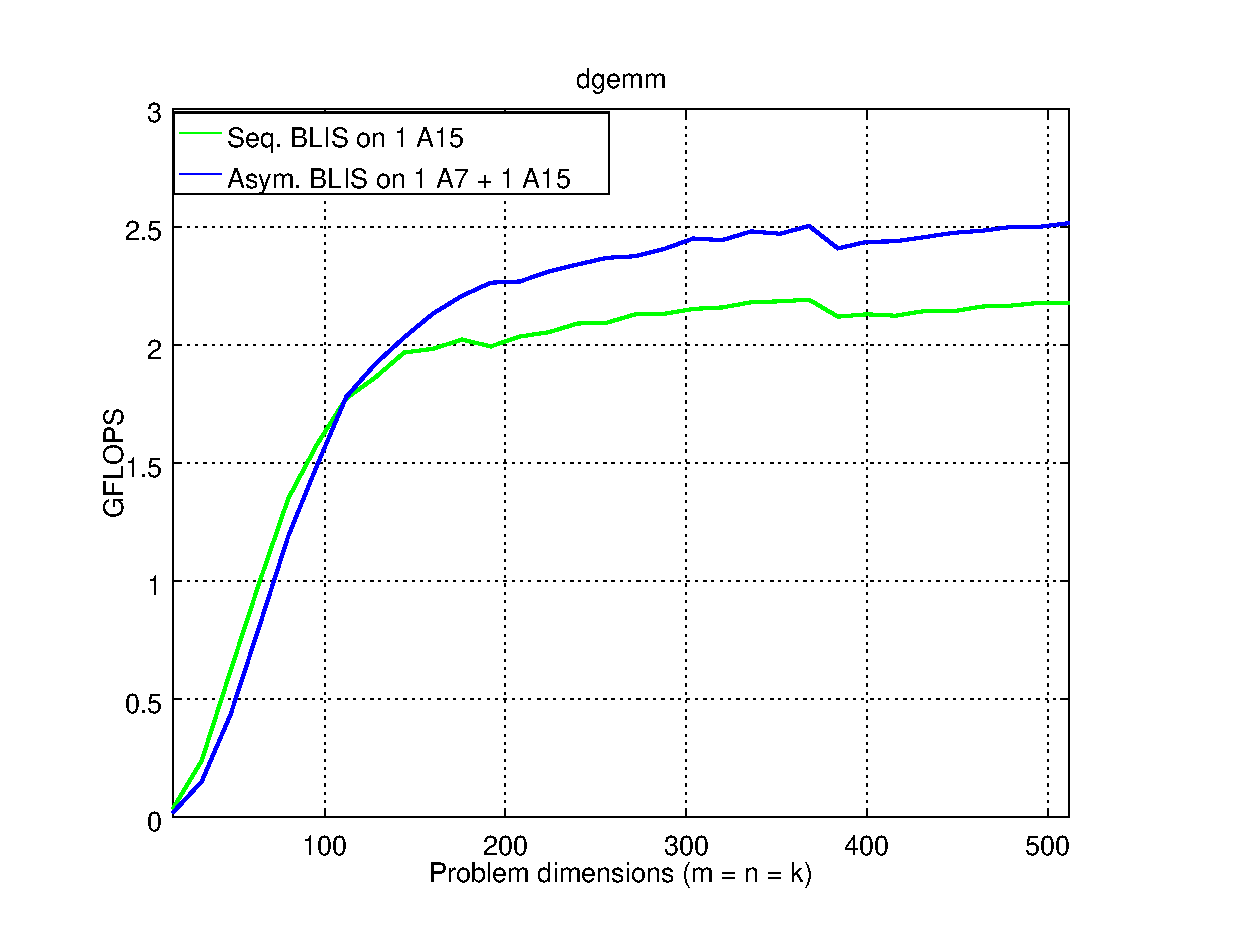
\includegraphics[width=0.49\textwidth]{Plots/BLIS_small/blis_dgemm_sym_asym}
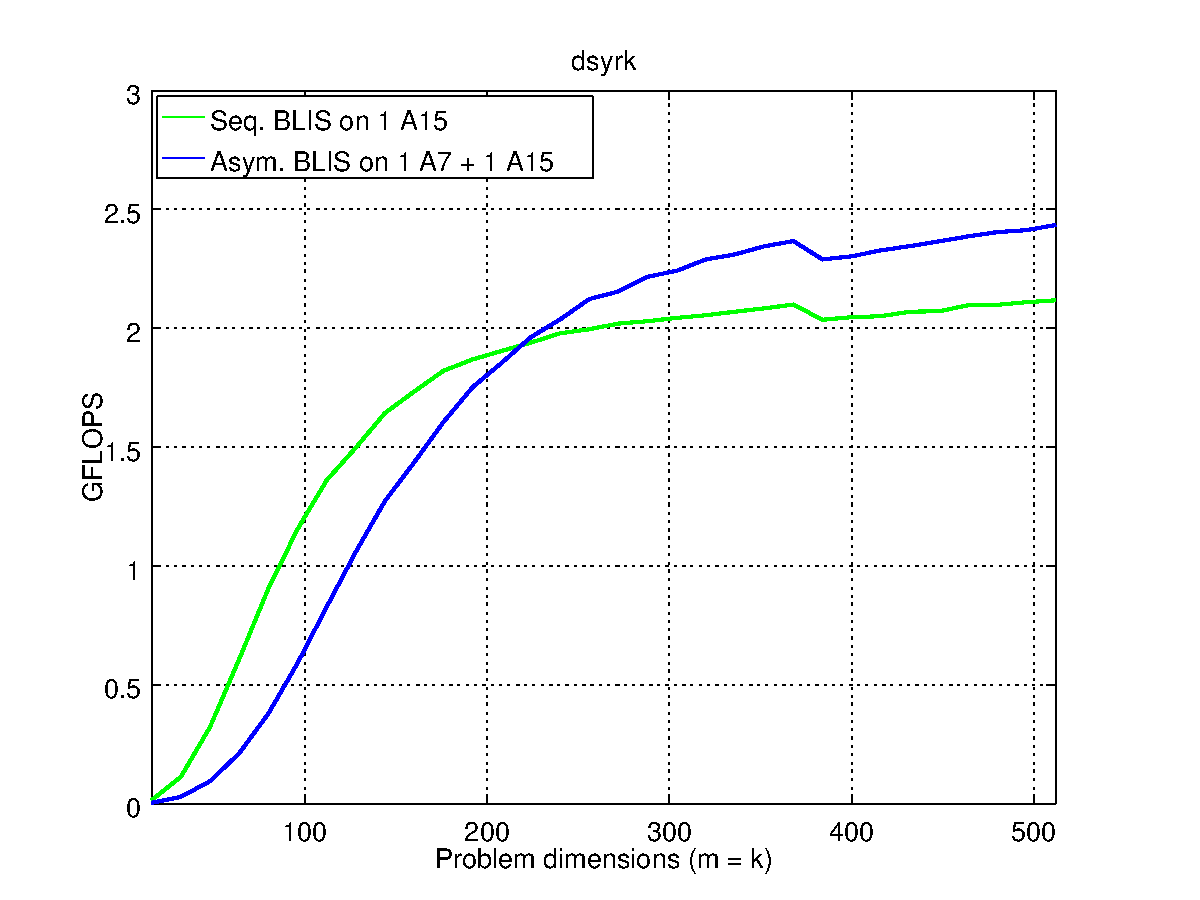
\includegraphics[width=0.49\textwidth]{Plots/BLIS_small/blis_dsyrk_sym_asym}
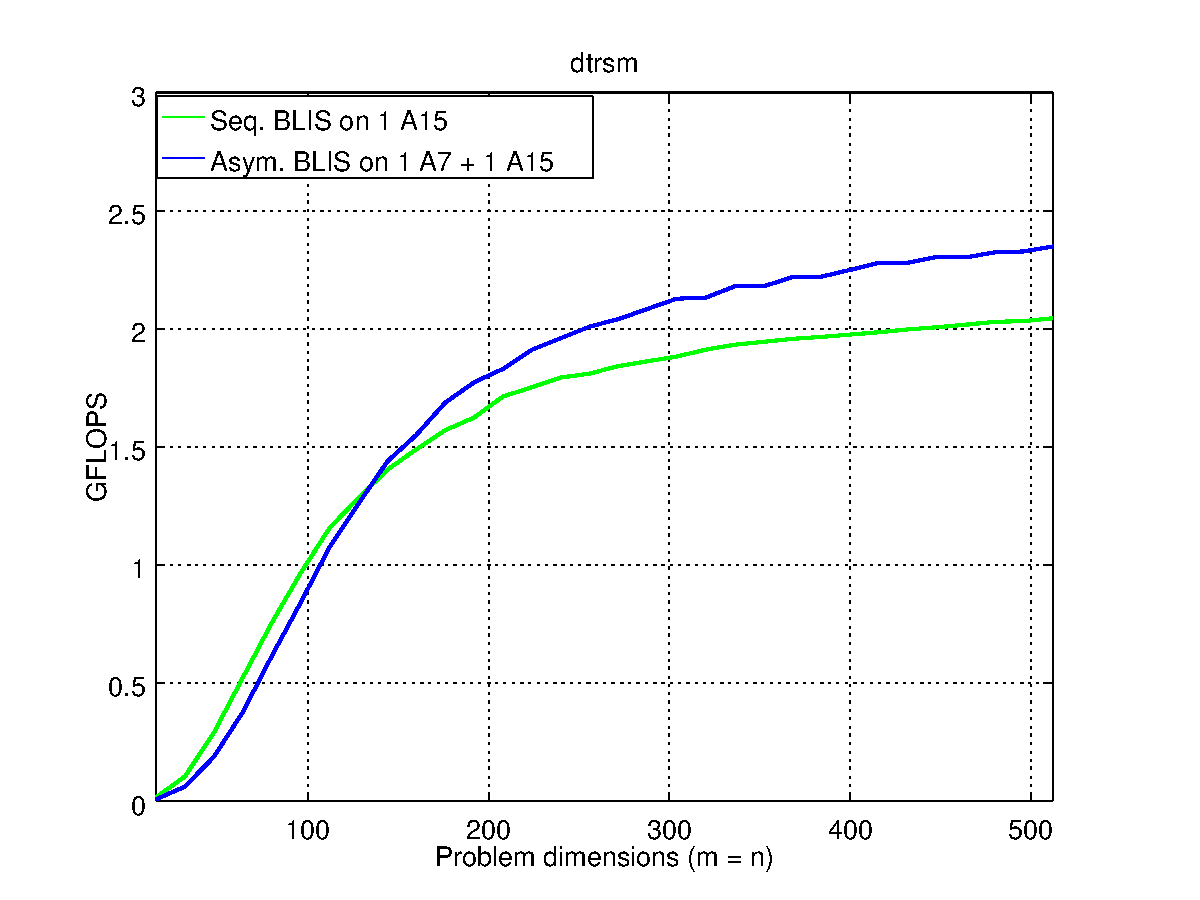
\includegraphics[width=0.49\textwidth]{Plots/BLIS_small/blis_dtrsm_sym_asym}
\caption{Performance of the BLAS-3 kernels in the sequential and the multi-threaded/asymmetric implementations of
         BLIS, using respectively one Cortex-A15 core and one Cortex-A15 plus one Cortex-A7 core
         of the Exynos 5422 SoC.}
\label{fig:cross_blis}
\end{figure}


\subsection{Integration of asymmetric BLIS in a conventional task scheduler}

%\begin{itemize}
	%\item En esta seccion comparamos runtime convencional, usando BLIS secuencial (1--4 worker threads OmpSs) y BLIS asimetrico (1+1 cores) por debajo del runtime. 
	%\item Mostrar rendimiento de ambas soluciones usando 1--4 worker threads.
	%\item Incidir en el aumento de rendimiento. En las tablas mostramos rendimiento neto ganado por nuestra solucion, y rendimiento por core anyadido. Este ultimo deberia
		%estar en el orden del rendimiento ganado por BLIS asimetrico contra BLIS simetrico mostrado en las graficas de la Figura~\ref{fig:cross_blis}.
%\end{itemize}

In order to analyze the actual benefits of our proposal, we next evaluate the conventional 
OmpSs task scheduler linked with either the sequential implementation of BLIS or its multi-threaded asymmetry-aware version. 
Hereafter, the BLIS kernels from first configuration always run using one Cortex-A15 core while, in the second case,
they exploit one Cortex-A15 plus one Cortex-A7 core.
%
Figure~\ref{fig:ompss_blis} reports the results for both setups, using an increasing number 
of worker threads from~1 to~4. For simplicity, we only report the results obtained with the optimal block size. 
In all cases, the solution based on the multi-threaded asymmetric library outperforms the sequential implementation for 
relatively large matrices (usually for dimensions {\tt n}~$>$~2,048) while, for smaller problems, the GFLOPS rates are 
similar. The reason for this behavior can be derived from the optimal block sizes reported in  
Table~\ref{tab:optimal_bs_sym} and the performance of BLIS reported in Figure~\ref{fig:cross_blis}: for that range 
of problem dimensions, the optimal block size is significantly smaller, and both BLIS implementations attain similar
performance rates.

\begin{figure}[t]
\centering
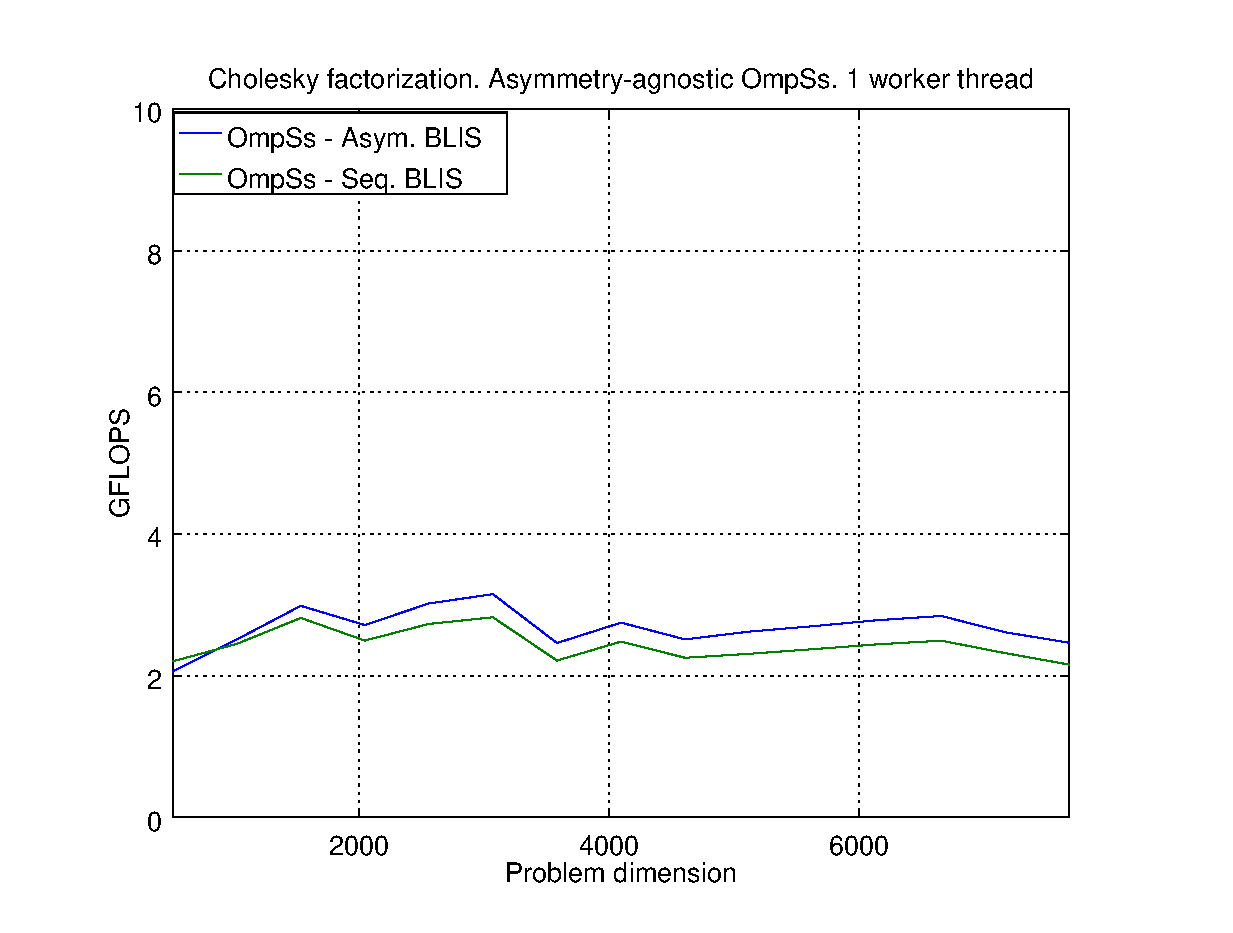
\includegraphics[width=0.49\textwidth]{Plots/Orig_runtime/plot_1_th}
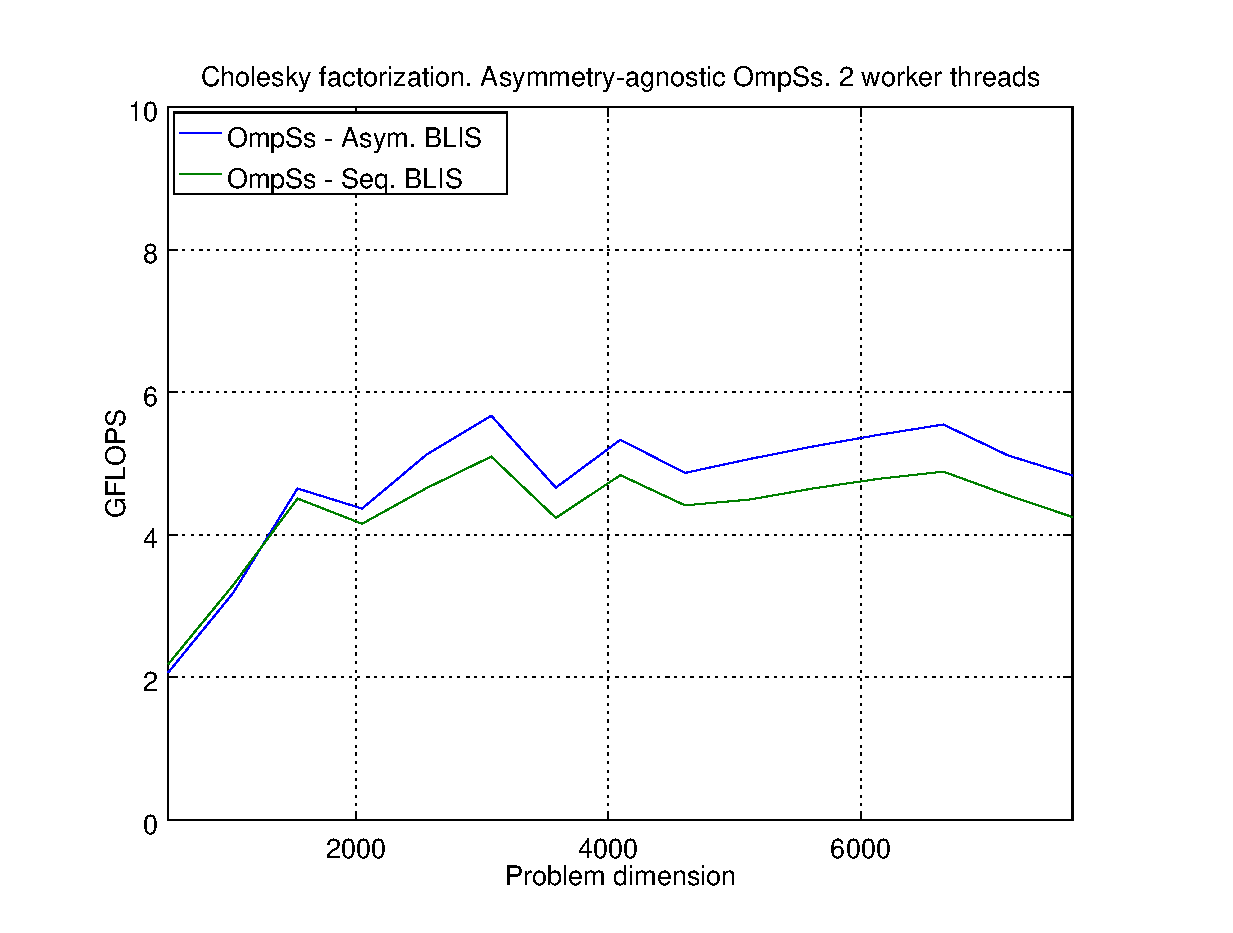
\includegraphics[width=0.49\textwidth]{Plots/Orig_runtime/plot_2_th}
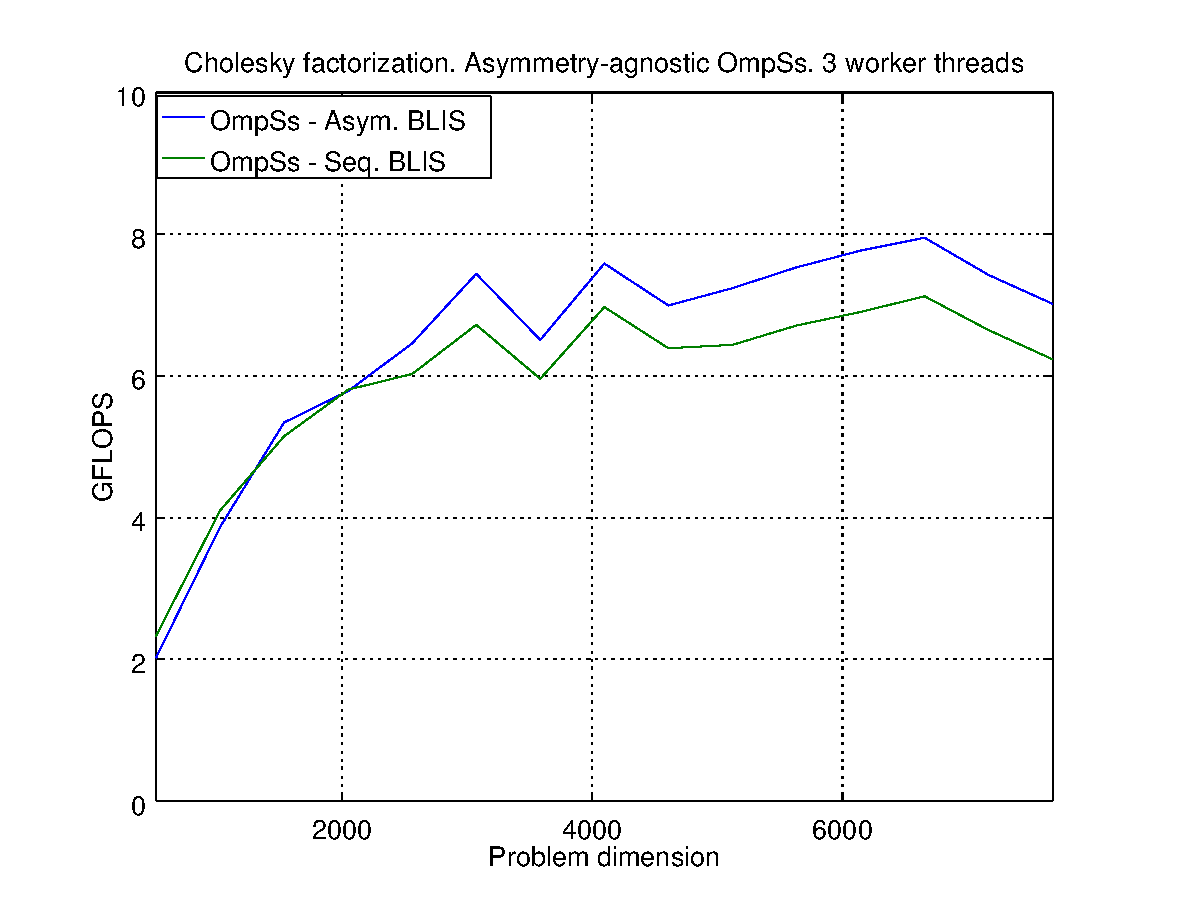
\includegraphics[width=0.49\textwidth]{Plots/Orig_runtime/plot_3_th}
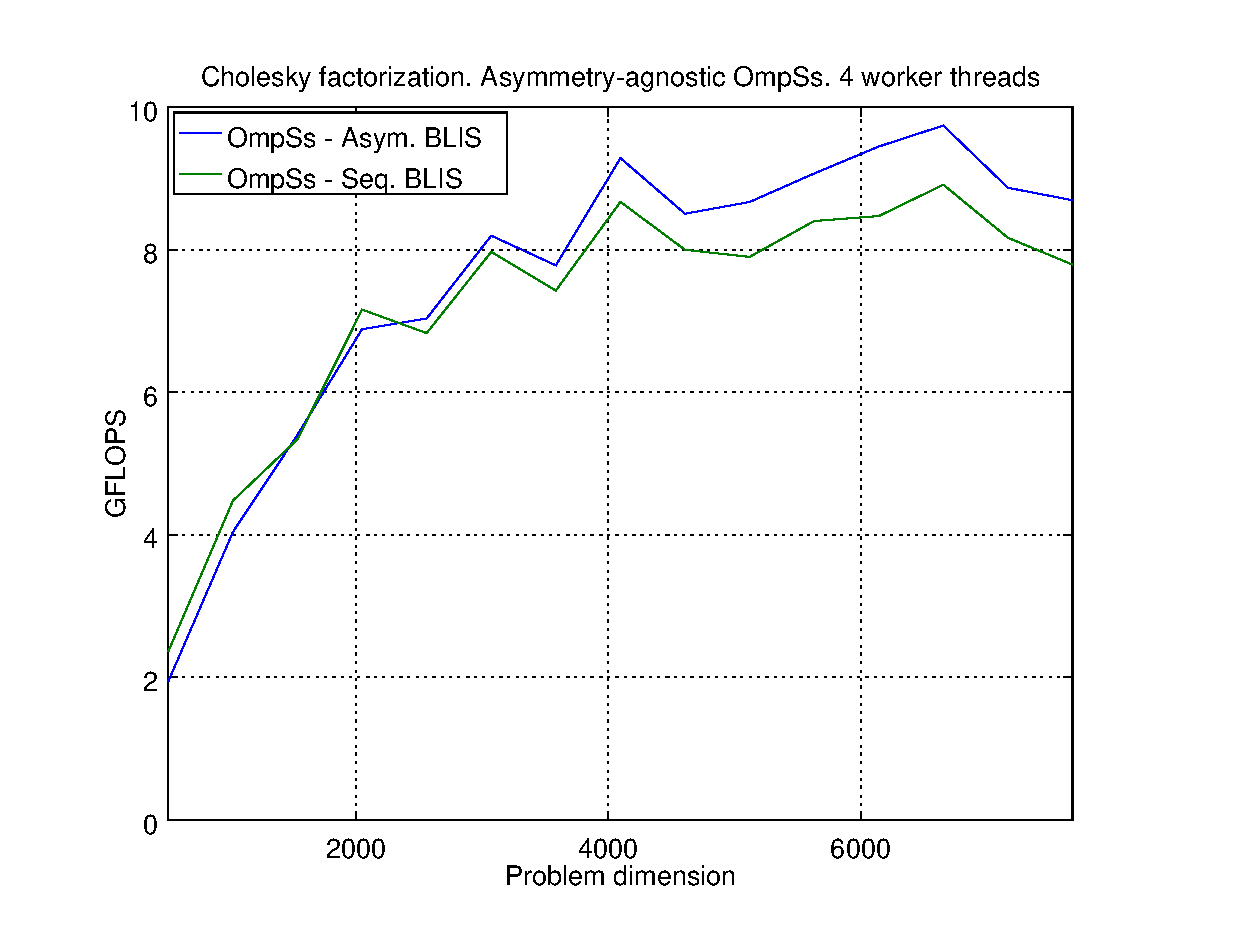
\includegraphics[width=0.49\textwidth]{Plots/Orig_runtime/plot_4_th}
\caption{Performance of the Cholesky factorization using the conventional OmpSs runtime linked with either
         the sequential or the multi-threaded/asymmetric implementations of
         BLIS %, using respectively one Cortex-A15 core and one Cortex-A15 plus one Cortex-A7 core,
         in the Exynos 5422 SoC.}
\label{fig:ompss_blis}
\end{figure}


%Table~\ref{tab:optimal_bs_sym}\ldots
%
%\begin{table}
	%\centering
	%\caption{Optimal block sizes for the Cholesky factorization using asymmetric BLIS.}
	%\label{tab:optimal_bs_asym}
	%\begin{tabular}{|c||c|c|c|c|c|c|c|c|c|c|c|c|c|c|c|}
		%\hline
		 %Th. &    512 & 1024 & 1536 & 2048 & 2560 & 3072 & 3584 & 4096 & 4608 & 5120 & 5632 & 6144 & 6656 & 7168 & 7680 \\ \hline \hline
		 %1   &    192 & 384 & 320 & 448 & 448 & 448 & 384 & 320 & 448 & 448 & 448 & 448 & 448 & 384 & 448 \\ \hline
		 %2   &    192 & 192 & 320 & 320 & 448 & 448 & 384 & 320 & 320 & 448 & 448 & 448 & 448 & 384 & 448 \\ \hline
		 %3   &    192 & 192 & 320 & 192 & 384 & 448 & 384 & 320 & 320 & 448 & 448 & 448 & 448 & 384 & 448 \\ \hline
		 %4   &    192 & 192 & 320 & 192 & 384 & 320 & 320 & 320 & 320 & 448 & 448 & 448 & 448 & 384 & 448 \\ \hline
	%\end{tabular}
%
%\end{table}

The quantitative difference in performance between both approaches is
reported in Tables~\ref{tab:improvement_absolute} and~\ref{tab:improvement_percore}. 
%In both tables, we
%report the difference in performance introduced by the use of an asymmetric BLIS implementation compared with the same setup using sequential BLIS. Table~\ref{tab:improvement_absolute} 
The first table illustrates the raw (i.e., absolute) gap, while the second
one shows the difference per Cortex-A7 core introduced in the experiment. 
Let us consider, for example, the problem size {\tt n}~=~6,144. 
In that case, the performance roughly improves by 0.975 GFLOPS when the 4~slow cores are added to help the base 4~Cortex-A15 cores. 
This translates into a performance raise of 0.243 GFLOPS per slow core, which is slightly under the 
improvement that could be expected from results experiments in the previous section. 
Note, however, that the performance per Cortex-A7 core is reduced from 0.340~GFLOPS, when adding just one
core, to 0.243~GFLOPS, when simultaneously using all four slow cores.

\newcommand{\fg}[1]{\textcolor{ForestGreen}{#1}} % Verde
\newcommand{\br}[1]{\textcolor{BrickRed}{#1}} % Rojo

\begin{table}
	\centering
\caption{Absolute performance improvement (in GFLOPS) for the Cholesky factorization using
         the conventional OmpSs runtime linked with 
         the multi-threaded/asymmetric BLIS with respect to the same runtime linked with the sequential BLIS in
         the Exynos 5422 SoC.}
	 \label{tab:improvement_absolute}

%\begin{tabular}{|c||c|c|c|c|c|c|c|c|c|c|c|c|c|} 
   	%\hline
	%Th. &        512    & 1024       & 2048     & 2560     & 3072      & 4096     & 4608     & 5120    & 5632    & 6144     & 6656     & 7168     & 7680 \\ \hline \hline
	%1   &     -0.143    & 0.061      & 0.218    & 0.289    & 0.326     & 0.267    & 0.259    & 0.313   & 0.324   & 0.340    & 0.348    & 0.294    & 0.300    \\ \hline
	%2   &     -0.116    & -0.109     & 0.213    & 0.469    & 0.573     & 0.495    & 0.454    & 0.568   & 0.588   & 0.617    & 0.660    & 0.558    & 0.582    \\ \hline
	%3   &     -0.308    & -0.233     & -0.020   & 0.432    & 0.720     & 0.614    & 0.603    & 0.800   & 0.820   & 0.866    & 0.825    & 0.777    & 0.78    \\ \hline
	%4   &     -0.421    & -0.440     & -0.274   & 0.204    & 0.227     & 0.614    & 0.506    & 0.769   & 0.666   & 0.975    & 0.829    & 0.701    & 0.902    \\ \hline
%\end{tabular}
%%\end{table}

\ra{1.2}
\ca{2pt}

{\scriptsize
\begin{tabular}{crrrrrrrrrrrrr} 
   	\toprule
                 & \phantom{a} & \multicolumn{12}{c}{Problem dimension ({\tt n})} \\ 
\cmidrule{3-14} 
     & \phantom{a} &       512      & 1,024        & 2,048          & 2,560        & 3,072        & 4,096        & 4,608        & 5,120        & 5,632        & 6,144        & 6,656         & 7,680 \\ \hline 
{\sc 1 wt} & \phantom{a} &    \br{-0.143} & \fg{0.061}  & \fg{0.218}    & \fg{0.289}  & \fg{0.326}  & \fg{0.267}  & \fg{0.259}  & \fg{0.313}  & \fg{0.324}  & \fg{0.340}  & \fg{0.348}   & \fg{0.300} \\ \cline{3-14}
{\sc 2 wt} & \phantom{a} &    \br{-0.116} & \br{-0.109} & \fg{0.213}    & \fg{0.469}  & \fg{0.573}  & \fg{0.495}  & \fg{0.454}  & \fg{0.568}  & \fg{0.588}  & \fg{0.617}  & \fg{0.660}   & \fg{0.582} \\ \cline{3-14}
{\sc 3 wt} & \phantom{a} &    \br{-0.308} & \br{-0.233} & \br{-0.020}   & \fg{0.432}  & \fg{0.720}  & \fg{0.614}  & \fg{0.603}  & \fg{0.800}  & \fg{0.820}  & \fg{0.866}  & \fg{0.825}   & \fg{0.780} \\ \cline{3-14}
{\sc 4 wt} & \phantom{a} &    \br{-0.421} & \br{-0.440} & \br{-0.274}   & \fg{0.204}  & \fg{0.227}  & \fg{0.614}  & \fg{0.506}  & \fg{0.769}  & \fg{0.666}  & \fg{0.975}  & \fg{0.829}   & \fg{0.902} \\ \bottomrule
\end{tabular}
}
\end{table}


%\begin{table}
	%\centering
	%\caption{Performance improvement per introduced core (in GFLOPS) when using asymmetric BLIS combined with OmpSs for the Cholesky factorization.}
	%\label{tab:improvement_percore}
%
%\begin{tabular}{|c||c|c|c|c|c|c|c|c|c|c|c|c|c|} 
   	%\hline
	 %Th. &       512    & 1024     & 2048     & 2560     & 3072      & 4096     & 4608     & 5120    & 5632     & 6144     & 6656    & 7168     & 7680 \\ \hline \hline
	 %1   &    -0.143    & 0.061    & 0.218    & 0.289    & 0.326     & 0.267    & 0.259    & 0.313   & 0.324    & 0.340    & 0.348   & 0.294    & 0.300    \\ \hline
	 %2   &    -0.058    & -0.054   & 0.106    & 0.234    & 0.286     & 0.247    & 0.227    & 0.284   & 0.294    & 0.308    & 0.330   & 0.279    & 0.291    \\ \hline
	 %3   &    -0.102    & -0.077   & -0.006   & 0.144    & 0.240     & 0.204    & 0.201    & 0.266   & 0.273    & 0.288    & 0.275   & 0.259    & 0.261    \\ \hline
	 %4   &    -0.105    & -0.110   & -0.068   & 0.051    & 0.056     & 0.153    & 0.126    & 0.192   & 0.166    & 0.243    & 0.207   & 0.175    & 0.225    \\ \hline
%\end{tabular}
%
%\end{table}


\begin{table}
\centering
\caption{Performance improvement per slow core (in GFLOPS) for the Cholesky factorization using
         the conventional OmpSs runtime linked with 
         the multi-threaded/asymmetric BLIS with respect to the same runtime linked with the sequential BLIS in
         the Exynos 5422 SoC.}
\label{tab:improvement_percore}

\ra{1.2}
\ca{2pt}
{\scriptsize
\begin{tabular}{crrrrrrrrrrrrr} 
   	\toprule
                 & \phantom{a} & \multicolumn{12}{c}{Problem dimension ({\tt n})} \\ 
\cmidrule{3-14} 
     & \phantom{a} &       512      & 1,024        & 2,048          & 2,560        & 3,072        & 4,096        & 4,608        & 5,120        & 5,632        & 6,144        & 6,656         & 7,680 \\ \hline 
	 {\sc 1 wt}    & \phantom{a} &    \br{-0.143} & \fg{0.061}  & \fg{0.218}  & \fg{0.289} & \fg{0.326}  & \fg{0.267} & \fg{0.259} & \fg{0.313} & \fg{0.324} & \fg{0.340} & \fg{0.348} & \fg{0.300}    \\ \cline{3-14}
	 {\sc 2 wt}    & \phantom{a} &    \br{-0.058} & \br{-0.054} & \fg{0.106}  & \fg{0.234} & \fg{0.286}  & \fg{0.247} & \fg{0.227} & \fg{0.284} & \fg{0.294} & \fg{0.308} & \fg{0.330} & \fg{0.291}    \\ \cline{3-14}
	 {\sc 3 wt}    & \phantom{a} &    \br{-0.102} & \br{-0.077} & \br{-0.006} & \fg{0.144} & \fg{0.240}  & \fg{0.204} & \fg{0.201} & \fg{0.266} & \fg{0.273} & \fg{0.288} & \fg{0.275} & \fg{0.261}    \\ \cline{3-14}
	 {\sc 4 wt}    & \phantom{a} &    \br{-0.105} & \br{-0.110} & \br{-0.068} & \fg{0.051} & \fg{0.056}  & \fg{0.153} & \fg{0.126} & \fg{0.192} & \fg{0.166} & \fg{0.243} & \fg{0.207} & \fg{0.225}    \\ \bottomrule
\end{tabular}
}

\end{table}

%% TABLAS ORIGINALES SIN SELECCIONAR COLUMNAS PARA QUE QUEPAN...
%\begin{table}
	%\centering
	%\caption{Absolute performance improvement (in GFLOPS) when using asymmetric BLIS combined with OmpSs for the Cholesky factorization.}
	%\label{tab:improvement_absolute}
%
%\begin{tabular}{|c||c|c|c|c|c|c|c|c|c|c|c|c|c|c|c|} 
   	%\hline
	%Th. &        512    & 1024     & 1536     & 2048     & 2560     & 3072     & 3584    & 4096     & 4608     & 5120    & 5632    & 6144     & 6656     & 7168     & 7680 \\ \hline \hline
	%1   &     -0.143    & 0.061    & 0.170    & 0.218    & 0.289    & 0.326    & 0.247   & 0.267    & 0.259    & 0.313   & 0.324   & 0.340    & 0.348    & 0.294    & 0.300    \\ \hline
	%2   &     -0.116    & -0.109   & 0.140    & 0.213    & 0.469    & 0.573    & 0.424   & 0.495    & 0.454    & 0.568   & 0.588   & 0.617    & 0.660    & 0.558    & 0.582    \\ \hline
	%3   &     -0.308    & -0.233   & 0.194    & -0.020   & 0.432    & 0.720    & 0.549   & 0.614    & 0.603    & 0.800   & 0.820   & 0.866    & 0.825    & 0.777    & 0.78    \\ \hline
	%4   &     -0.421    & -0.440   & 0.063    & -0.274   & 0.204    & 0.227    & 0.353   & 0.614    & 0.506    & 0.769   & 0.666   & 0.975    & 0.829    & 0.701    & 0.902    \\ \hline
%\end{tabular}
%\end{table}
%
%\begin{table}
	%\centering
	%\caption{Performance improvement per introduced core (in GFLOPS) when using asymmetric BLIS combined with OmpSs for the Cholesky factorization.}
	%\label{tab:improvement_percore}
%
%\begin{tabular}{|c||c|c|c|c|c|c|c|c|c|c|c|c|c|c|c|} 
   	%\hline
	 %Th. &       512    & 1024    & 1536    & 2048     & 2560     & 3072     & 3584    & 4096     & 4608     & 5120    & 5632     & 6144     & 6656    & 7168     & 7680 \\ \hline \hline
	 %1   &    -0.143    & 0.061   & 0.170   & 0.218    & 0.289    & 0.326    & 0.247   & 0.267    & 0.259    & 0.313   & 0.324    & 0.340    & 0.348   & 0.294    & 0.300    \\ \hline
	 %2   &    -0.058    & -0.054  & 0.070   & 0.106    & 0.234    & 0.286    & 0.212   & 0.247    & 0.227    & 0.284   & 0.294    & 0.308    & 0.330   & 0.279    & 0.291    \\ \hline
	 %3   &    -0.102    & -0.077  & 0.064   & -0.006   & 0.144    & 0.240    & 0.183   & 0.204    & 0.201    & 0.266   & 0.273    & 0.288    & 0.275   & 0.259    & 0.261    \\ \hline
	 %4   &    -0.105    & -0.110  & 0.015   & -0.068   & 0.051    & 0.056    & 0.088   & 0.153    & 0.126    & 0.192   & 0.166    & 0.243    & 0.207   & 0.175    & 0.225    \\ \hline
%\end{tabular}
%\end{table}

\subsection{Performance comparison versus asymmetry-aware task scheduler}
\label{sec:comparative}

Our last round of experiments aims to assess the performance advantages of different task-parallel executions
of the Cholesky factorization via OmpSs. Concretely, we consider 
(1) the conventional task scheduler linked with the sequential BLIS (``OmpSs - Seq. BLIS''); 
(2) the conventional task scheduler linked with our multi-threaded asymmetric BLIS that views the SoC as four symmetric {\em virtual cores}
(``OmpSs - Asym. BLIS''); and 
(3) the criticality-aware task scheduler in Botlev-OmpSs linked with the sequential BLIS
(``Botlev-OmpS - Seq. BLIS''). 
In the executions, we use all four Cortex-A15 cores and 
evaluate the impact of adding an increasing number of Cortex-A7 cores, from~1 to~4, for Botlev-OmpSs. 

Figure~\ref{fig:comparative} shows the performance attained by the aforementioned alternatives on the Exynos 5422 SoC.
The results can be divided into groups along three problem dimensions:
\begin{itemize}
 \item For small matrices ({\tt n}~=~512, 1,024), the conventional runtime using exclusively the four big cores (that is,
linked with a sequential BLIS library for task execution) attains the best results in terms of performance. This was
expected and was already observed in Figure~\ref{fig:ompss_blis}; the main reason is the small optimal block size,
enforced by the reduced problem size, that is necessary in order to expose enough task-level parallelism. This invalidates the
use of our asymmetric BLIS implementation due to the low performance for very small matrices;
see Figure~\ref{fig:cross_blis}. We note that the ad-hoc Botlev-OmpSs does not attain
remarkable performances either for this dimension range, regardless the amount of Cortex-A7 cores used.

 \item For medium-sized matrices ({\tt n}~=~2,048, 4,096), the gap in performance between the different approaches is reduced. 
The variant that relies on the asymmetric BLIS implementation commences to outperform the alternative implementations for
{\tt n}=4,096 by a short margin. For this problem range, Botlev-OmpSs is competitive, and also outperforms the conventional setup.

 \item For large matrices ({\tt n}~=~6,144, 7,680) this trend is consolidated, and both asymmetry-aware approaches deliver
remarkable performance gains with respect to the conventional setup. Comparing both asymmetry-aware solutions, our
mechanism attains better performance rate, even when considering the usage of all available cores for the Botlev-OmpSs
runtime version.

\end{itemize}

\begin{figure}
\centering
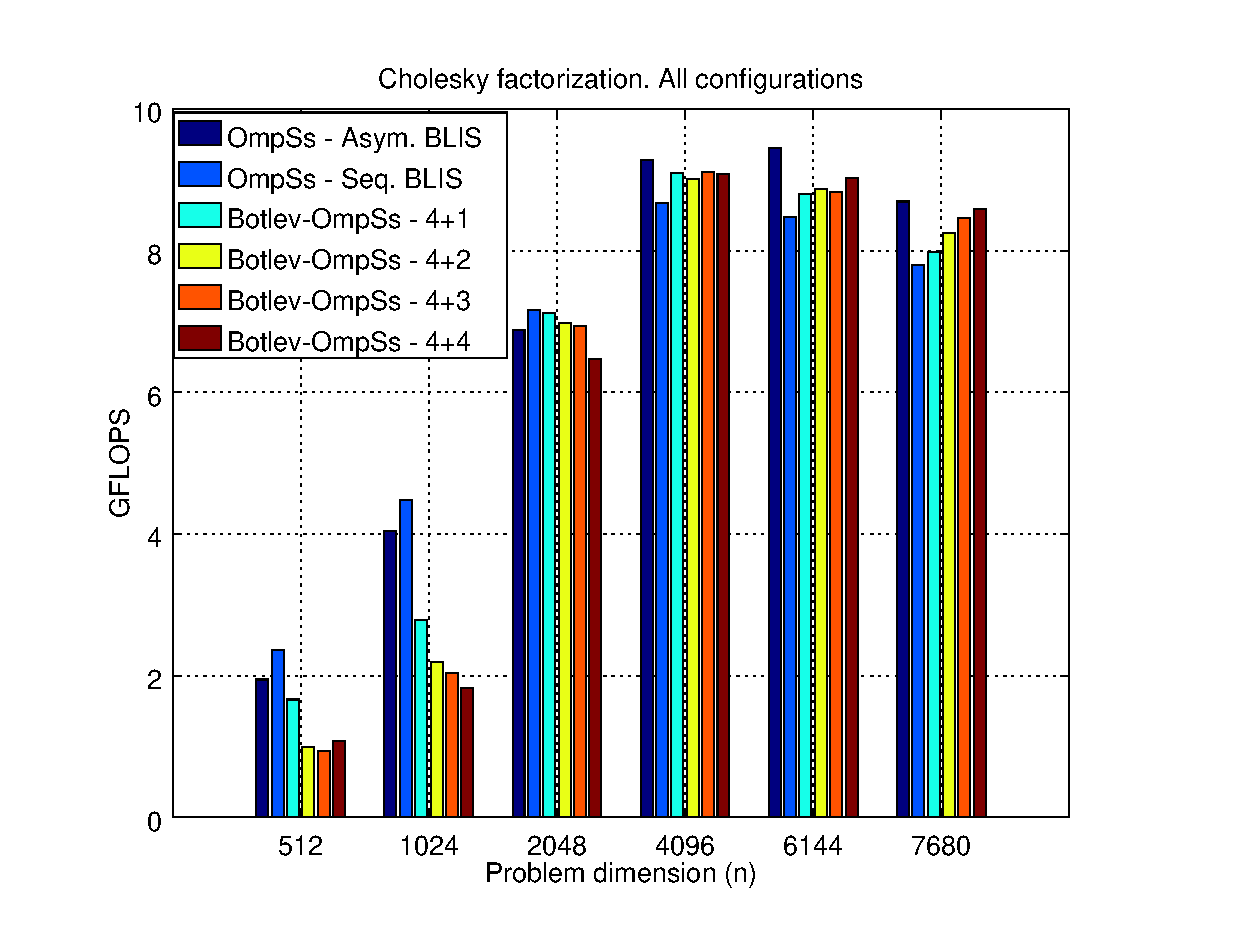
\includegraphics[width=0.70\textwidth]{Plots/Comparative/comparative}
\caption{Performance (in GFLOPS) for the Cholesky factorization using
         the conventional OmpSs runtime linked with 
         either the sequential BLIS or the multi-threaded/asymmetric BLIS, and the {\em ad-hoc} asymmetry-aware version of the
         OmpSs runtime (Botlev-OmpSs) linked with the sequential BLIS in 
         the Exynos 5422 SoC. The labels of the form ``4+x'' refer to an execution with 4 Cortex-A15 cores and x Cortex-A7 cores.}
\label{fig:comparative}
\end{figure}

To summarize, our proposal to exploit asymmetry improves portability and programmability by avoiding
a revamp of the runtime task scheduler for AMPs. In addition, our approach renders performance
gains which are, for all problems cases, comparable with those of ad-hoc asymmetry-conscious schedulers; 
for medium to large matrices, it clearly outperforms the efficiency attained with a conventional 
asymmetry-oblivious scheduler.


%-- Configuraciones para emacs --
%%% Local Variables:
%%% mode: latex
%%% TeX-master: "./principal.tex"
%%% End:
